%Select document class: 12 point, article
\documentclass[12pt]{article}

% This template is a combination of work done by Mike Catanzaro and Gabe Angelini-Knoll, both formerly of the WSU math dept, with some additions and synthesizations by Clayton Hayes (clayton.hayes@wayne.edu) for broader use
% Last updated 2018-03-10 by Aaron Willcock (ez9213@wayne.edu)

%AMS = American Mathematical Society
%math, symbols, theorems, fonts
\usepackage{amsmath, amssymb, amsthm, amsfonts}

%Enhanced graphics support (https://ctan.org/pkg/graphicx?lang=en)
\usepackage{graphicx}

%Set default graphics path (replace 'figures/' with whatever directory your images are in)
%\graphicspath{{figures/}}


%Control layout of itemize, enumerate, description (https://ctan.org/pkg/enumitem?lang=en)
\usepackage{enumitem}

% Header and footer formatting options
\usepackage{fancyhdr}

%Control float placement. [section] = "stop floats at section boundaries is to change the definition of “\section” to include “\FloatBarrier”"
\usepackage[section]{placeins}

%Hypertext (links) in LaTeX. [option] = remove color and border on links.
\usepackage[hidelinks]{hyperref}

%\usepackage[all]{xy}
%\usepackage{mathtools}

%Pro­gram­ming fa­cil­i­ties for LaTeX class and pack­age authors
\usepackage{etoolbox}

%Indent first paragraph of every 'chapter' aka section
\usepackage{indentfirst}

%Title formatting option. [explicit] = make titles all caps
\usepackage[explicit]{titlesec}

%Standard package for selecting font encodings. [T1] = Support for accented characters
%(https://texfaq.org/FAQ-why-inp-font) - 
%(https://tex.stackexchange.com/questions/664/why-should-i-use-usepackaget1fontenc)
\usepackage[T1]{fontenc}

%Charter fonts
\usepackage{charter}

%\usepackage[expert]{mathdesign}

%Control table of contents, figures, etc
\usepackage{tocloft}

%Set space between lines. [option] = Double/single spacing necessary for properly formatting ToC/LoFT and titles.
\usepackage[doublespacing]{setspace}

%Create normal/logarithmic plots in two and three dimensions
\usepackage{pgfplots}
%Request a specific version
\pgfplotsset{compat=1.5}

\newcommand\scalemath[2]{\scalebox{#1}{\mbox{\ensuremath{\displaystyle #2}}}}

%Modify section headers (aka chapters) to be: centered, single space, large, bold, preceded with the word 'CHAPTER 'and with 0.4 em of space before title 
\titleformat{\section}[block]{\centering\singlespace\large\bf}{CHAPTER \thesection \hspace{0.4em} \MakeUppercase{#1}}{0em}{}{}


%Modify unnumbered section headers (aka chapters) to be: centered, single space, large, bold, preceded with the word 'CHAPTER 'and with 0.4 em of space before title 
\titleformat{name=\section,numberless}[block]{\centering\singlespace\large\bf}{\hspace{0.4em} \MakeUppercase{#1}}{0em}{}{}

%Remove spacing left of, above, and below sections and subsections
% \titlespacing{command}{left spacing}{before spacing}{after spacing}[right] (https://tex.stackexchange.com/questions/53338/reducing-spacing-after-headings)
\titlespacing{\section}{0pt}{0pt}{0pt}
\titlespacing{\subsection}{0pt}{0pt}{0pt}
\titlespacing{\subsubsection}{0pt}{0pt}{0pt}

% Modify TOC entries with tocloft: insert the word 'Chapter ' and then add 6em of space after the word
\renewcommand{\cftsecleader}{\cftdotfill{\cftdotsep}}
\renewcommand{\cftsecpresnum}{Chapter }
\cftsetindents{section}{0em}{6em}

% Call the other parts of the document 'part' and make the table of contents print them correctly
\renewcommand{\cftpartfont}{}
\renewcommand{\cftpartpagefont}{}
\renewcommand{\cftpartleader}{\cftdotfill{\cftdotsep}}
\renewcommand{\cftbeforepartskip}{0em}
\renewcommand{\cftpartindent}{1.5em}

% Change spacing above chapters in toc, remembering that they are really sections
\setlength{\cftbeforesecskip}{0em}

% Adds space after ToC entries to make them appear double-spaced
\renewcommand\cftsecafterpnum{\vskip\baselineskip}
\renewcommand\cftsubsecafterpnum{\vskip\baselineskip}
\renewcommand\cftsubsubsecafterpnum{\vskip\baselineskip}
\renewcommand\cftpartafterpnum{\vskip\baselineskip}

%Add space after LoF entries to make them appear double-spaced
\renewcommand\cftfigafterpnum{\vskip\baselineskip}

%Add space after LoT entries to make them appear double-spaced
\renewcommand\cfttabafterpnum{\vskip\baselineskip}

% Remove the extra space above and below theorems, lemmas, props, etc. The important point in the following is the  0pt preskip and the 0pt postskip
\makeatletter
\def\thm@space@setup{\thm@preskip=0pt
\thm@postskip=0pt}
\makeatother
\newtheoremstyle{newstyle}      
{} % Aboveskip 
{} % Below skip
{\mdseries} % Body font e.g.\mdseries,\bfseries,\scshape,\itshape
{} % Indent
{\bfseries}  % Head font e.g.\bfseries,\scshape,\itshape
{.} % Punctuation afer theorem header
{ } % Space after theorem header
{} % Heading

% The above does not fix the spacing around proof environments so use the following; the crucial point is the topsep0\p@, i.e., topsep = 0 pt. The rest is essentially copied from the standard AMS environment.
\makeatletter
\renewenvironment{proof}[1][\proofname]{\par
  \pushQED{\qed}%
  \normalfont \topsep0\p@\relax
  \trivlist
  \item[\hskip\labelsep\itshape
  #1\@addpunct{.}]\ignorespaces 
}{
  \popQED\endtrivlist\@endpefalse
}
\makeatother

% Fix bibliography heading
% \makeatletter
% \renewenvironment{thebibliography}[1]{%
%   \@xp\section\@xp*\@xp{\refname}%
%   \normalfont\footnotesize\labelsep .5em\relax
%   \renewcommand\theenumiv{\arabic{enumiv}}\let\p@enumiv\@empty
%   \vspace*{-35pt}% NEW
%   \list{\@biblabel{\theenumiv}}{\settowidth\labelwidth{\@biblabel{#1}}%
%     \leftmargin\labelwidth \advance\leftmargin\labelsep
%     \usecounter{enumiv}}%
%   \sloppy \clubpenalty\@M \widowpenalty\clubpenalty
%   \sfcode`\.=\@m
% }{%
%   \def\@noitemerr{\@latex@warning{Empty `thebibliography' environment}}%
%   \endlist
% }
% \makeatother

%Remove default "References" text from \bibliography call
\patchcmd{\thebibliography}{\section*{\refname}}{}{}{}

%Remove spacing between bibliography entries
%   Set "OLDthebibliography" to be "thebibliography"
\let\OLDthebibliography\thebibliography
%   Renew command with 0pt spacing for paragraph and item separation
\renewcommand\thebibliography[1]{
    \OLDthebibliography{#1}
    \setlength{\parskip}{0pt}
    \setlength{\itemsep}{0pt plus 0.3ex}
}

% Formatting
\usepackage[left=1in,right=1in, top=1in, bottom=1in]{geometry}
\renewcommand{\arraystretch}{0.85}
\renewcommand{\baselinestretch}{2}
\renewcommand{\headrulewidth}{0pt}

\newcommand{\Mdef}[2]{\newcommand{#1}{\relax \ifmmode #2 \else $#2$\fi}}

% Spacing commands, which may or may not be used in the following.
\newcommand{\one}{{\rm \bf1}\hspace*{-0.035in} {\rm l}}
\newcommand{\nd}{\noindent}
\def\para#1{\vskip 0.4\baselineskip\noindent{\bf #1}}
\newcommand{\Vspc}{\vspace*{0.1in}}

\newcommand{\ID}{\index}
\makeatletter \@addtoreset{equation}{section} \makeatother

%Section Labeling
\renewcommand{\thesection}{\arabic{section}}

%Equation Numbering Ex. Section 3, Equation 2 = Equation 3.2
\renewcommand{\theequation}{\thesection.\arabic{equation}}

\renewcommand{\cftsecfont}{}
\renewcommand{\cftsecpagefont}{}

%List of Tables edits
\renewcommand{\cfttabpresnum}{Table }
\renewcommand{\cfttabindent}{1.0em}
\renewcommand{\cfttabnumwidth}{5.0em}

%List of Figures edits
\renewcommand{\cftfigpresnum}{Figure }
\renewcommand{\cftfigindent}{1.0em}
\renewcommand{\cftfignumwidth}{5.5em}

% \usepackage{etoolbox}
% \makeatletter
% \patchcmd{\@caption}{\csname the#1\endcsname}{\csname fnum@#1\endcsname:}{}{}
% \makeatother

%%%%%%%%%%%%%%%%%%%%%%%%%%%%%%%%%%%%%%%%%%%%%%%%%%%%%%%%%%%%%%%%%%%%%

\begin{document}

% \makeatletter
% \renewcommand\l@figure{\@dottedtocline{1}{1.0em}{5.5em}}
% \renewcommand\l@table{\@dottedtocline{1}{1.0em}{5.0em}}
% \makeatother

\centerline{\bf TRADING UTILIZATION FOR CIRCUITRY}
\vspace{-0.4cm}
\centerline{\bf HARDWARE-SOFTWARE CO-DESIGN FOR REAL-TIME}
\vspace{-0.4cm}
\centerline{\bf SOFTWARE-BASED SHORT-CIRCUIT PROTECTION}

\vskip-0.4cm

\thispagestyle{empty}

\begin{center}
    \vspace{-0.4cm}
    by \\
    %\Vspc
    {\bf AARON WILLCOCK}\\ % Name here
    %\Vspc
    {\bf THESIS}\\
    %\Vspc
    Submitted to the Graduate School,\\
    of Wayne State University,\\
    Detroit, Michigan\\
    in partial fulfillment of the requirements\\
    for the degree of\\
    %\Vspc
    {\bf MASTER OF SCIENCE}
\end{center}

\begin{flushleft}
    \vspace*{-0.20in}
    \hspace*{3.09in}2019 % Year here
    \hspace*{3.09in}MAJOR: COMPUTER SCIENCE\\ % Major here
    %\Vspc
    \hspace*{3.09in}Approved By:\\
    %\Vspc
    \hspace*{3.09in}-----------------------------------------------------------\\
    \vspace*{-0.25in}
    \hspace*{3.09in}Advisor\hspace*{1.5in} Date\hspace*{0.1in}\\
    %\bigskip
    %\hspace*{3.09in}-----------------------------------------------------------\\
    %\medskip
    %\hspace*{3.09in}-----------------------------------------------------------\\
    %\medskip
    %\hspace*{3.09in}-----------------------------------------------------------\\
    %\medskip
    %\hspace*{3.09in}-----------------------------------------------------------
\end{flushleft}

\newpage

\pagestyle{fancy} \chead{} \rhead{} \lhead{}
\pagenumbering{roman} \lfoot{}\cfoot{\thepage}\rfoot{}
\setcounter{page}{2}

\section*{DEDICATION}
\addcontentsline{toc}{section}{Dedication}
\begin{center}
To Ellen, Kevin, Sue, Carina, and Connor.
\end{center}

\newpage

\section*{ACKNOWLEDGEMENTS}
\addcontentsline{toc}{section}{Acknowledgements}
\begin{center}
This research has been supported in part by: \\
the US National Science Foundation (CNS Grant Nos. 0953585, 1205338,  \& 1618185)\\ and a Thomas C. Rumble Graduate Fellowship from Wayne State University.\par
\end{center}
\newpage

\begin{singlespace}
\renewcommand{\contentsname}{\hfill\large TABLE OF CONTENTS \hfill}
\tableofcontents
\newpage
\addcontentsline{toc}{section}{List of Tables}
\renewcommand{\listtablename}{\hfill\large LIST OF TABLES \hfill}
\listoftables
\newpage
\addcontentsline{toc}{section}{List of Figures}
\renewcommand{\listfigurename}{\hfill\large LIST OF FIGURES \hfill}
\listoffigures
\end{singlespace}

\clearpage

\pagestyle{fancy} \chead{\thepage} \rhead{} \lhead{}
\pagenumbering{arabic} \lfoot{}\cfoot{}\rfoot{}
\setcounter{equation}{0}

\clearpage \section{Introduction}		\label{chap:Introduction}

\subsection{Motivation and Applications}
From cell phones to solar panels, devices of all sizes require power semiconductors to control, direct, and manage the flow of electricity.
Batteries, CPUs, and photovoltaic inverters all leverage this flow of electricity, known as current, to perform tasks from actuation to computation.
In excess, however, current leads to thermal cycling and can be degrading or destructive to power circuitry.
One cause of excessive current is short-circuiting.
A short-circuit occurs when current travels through an alternate, unintended path in a circuit often with little or no resistance.
This alternate path of travel with no resistance leads to high current, increased heat, and often circuit damage.
This potential for damage creates a need for short-circuit protection.

The need for short protection can be seen in a variety of applications relying on power semiconductors including power converters and inverters \cite{hiSpeedProtection}.
In an industrial setting, this can include photovoltaic systems and hybrid fuel cells \cite{photoVoltaic}. 
In a consumer setting, this can include cell phones and other portable electronics like the recent Samsung Galaxy Note 7 which was recalled due to fires caused by short-circuits in the device battery \cite{explodingPhone}.

To mitigate the risk of short-circuits, devices using power-semiconductors can be constructed with short-circuit protection in the form of a fuse, thermal breaker, or other hardware designated to prevent the high current responsible for circuit damage. 
This short-circuit protection, however, is often fixed circuitry dedicated solely to short detection. In such systems, little flexibility is afforded to circuits which operate at varying voltages and currents over their lifetime as designers must protect against short-circuits at the highest currents and voltages, even if they are not the most frequently used. Moreover, the rise in semiconductor power density continues to reduce the required latency for detecting and halting shorts \cite{gateChargeChara}.

\subsection{Problem Statement}
In light of the motivation above, the problem of designing flexible short-circuit protection systems can be viewed through the lens of real-time software.
Given the inherent possibility of catastrophic failure in short-circuit protection systems and the time-sensitive nature of current rise during short-circuits, we seek to frame the problem as one of hardware-software co-design via hard real-time systems.
Specifically, we aim to address the problem of short-circuit protection in direct current (DC) resistor-inductor (RL) circuits - circuits containing resistors and inductors where current flows in only one direction.

To address the need for flexible, short-circuit protection, our problem statement is:

\noindent Given a Direct-Current Resistor-Inductor circuit, devise a hardware-software co-design approach which relates hard-real time requirements to hardware size. More specifically, our objective is to construct a hardware-software relationship which allows designers to:
\begin{enumerate}
    \item minimize hardware size while meeting maximum real-time utilization requirements, and
    \item minimize real-time utilization while meeting maximum hardware size requirements.
\end{enumerate}

\subsection{Proposed Solution}
To address the need for flexible, real-time short-circuit protection, we propose a short-protection method via a real-time task as follows:

A DC RL circuit containing an air-core inductor placed in series between the system's resistive load and ground has is connected (and controlled) by a microcontroller.The microcontroller executes a real-time task responsible for sampling voltage across the inductor (or a small resistor) to measure current via an Analog-to-Digital Converter (ADC) pin. Short protection is accomplished by identifying the maximum expected current and the maximum rate of current change as limited by the circuit's inductor. Using the inductor spatial parameters in conjunction with ADC sampling times, a minimum sampling period is derived for the real-time task. From this minimum period, a relationship between minimum real-time utilization under Earliest Deadline First (EDF) scheduling and inductor volume  is provided. Real-time or physical system constraints may be applied to this relationship to facilitate the hardware-software co-design of a real-time short-circuit protection system.

This approach is intended to allow existing systems with microprocessors to migrate short-circuit protection from dedicated-circuitry-only to a software-based implementation and future systems to be designed with the proposed hardware-software tradeoff in mind.

\subsection{Contributions}
%Contributions: Long-form writing
The software-based protection methods depicted herein provide an alternative short-circuit protection technique to circuit designers. By relating utilization to the volume of (and board space consumed by) an inductor, system designers may trade short-protection circuitry for real-time task utilization on the microcontroller, leveraging either end of the relationship to meet fault-tolerance and space requirements. For example, applications with little available board space may opt for smaller inductors (minimizing board space) and greater utilization. Example applications include smaller IGBT modules as found in electric vehicles or applications where minimizing weight is import\cite{IGBTvehicle}. In contrast, larger applications with more available board space or a greater real-time task set may opt for a larger inductor and thus a smaller utilization for the short-protection task. Example applications include high power IGBT modules in photovoltaic and wind turbine inverters \cite{photoVoltaic}\cite{hiPowerIGBTwind}. Perhaps most importantly, the established relationship between board space and processor utilization acts as a conduit through which advancements in electrical engineering may improve real-time system efficiency and vice versa.
To summarize, our contributions include\footnote{This work was published in the 2017 IEEE 23rd International Conference on Embedded and Real-Time Computing Systems and Applications (RTCSA) under the same title \cite{tufc} and is an extension upon the related senior thesis by Willcock \cite{seniorThesis}.}:%Contributions: Bullet-point summary
\begin{description}
\item [1.] a software-based short protection method for Direct Current Resistor-Inductor circuits,
\item [2.] a relationship between air-core inductor spatial parameters and real-time processor utilization under preemptive uniprocessor EDF scheduling for short-circuit protection,
\item [3.] a process for identifying optimal inductor orientation given a fixed volume, and
\item [4.] a process for minimizing utilization given a fixed volume for an air-core inductor and vice versa.
%\item [5.] A process for minimizing the required volume for an air-core inductor given a fixed utilization.
\end{description}


%Outline of paper
\subsection{Outline}
Chapter \ref{chap:related work} details the related work in both problem domains.
Chapter \ref{chap:electronics background} provides an electronics background and nomenclature overview.
Chapter \ref{chap:electronic system model} provides the first paper contribution, a model for identifying circuit properties.
Chapter \ref{chap:method of protection} depicts short protection methods given the constraints provided in the circuit model.
Chapter \ref{chap:real-time system model} formalizes the relation between real-time scheduling and short-circuit protection.
Chapter \ref{chap:model optimization} provides the model optimization for both fixed board constraints and fixed real-time utilization as contributions from this paper.
Chapter \ref{chap:experiments} details experiments conducted to validate the proposed relationship and theoretical utilization.
Chapter \ref{chap:results} discusses the results of experimentation.
Chapter \ref{chap:conclusion} identifies conclusions and future work.

%Intersection of EE and RTS
%The problem of protecting electronics from short-circuits has traditionally been a concern of electrical engineering and has been addressed through several techniques including current mirrors and clamp circuits \cite{litRev}. With the application of real-time software to short protection, we shift the problem to the intersection of electrical engineering, cyber-physical, and real-time systems. Thus, solutions are subject to the physical, electronic, and real-time limitations of the system.

%The proposed software-based short-circuit protection approach aims to reduce dedicated circuitry on platforms already using a microprocessor and provide an alternative method to short protection. The motivation behind this hardware-software co-design approach is the flexibility and ubiquity of microprocessors. The potential for movement of protection systems from dedicated circuitry to software implementations. [OLD]


\clearpage \section{Related Work}  \label{chap:related work}

To the best of our knowledge, current approaches to short-circuit protection are rooted in dedicated circuitry and do not use adaptive real-time processing. Modern methodologies include Zone Selective Interlocking on systems with alternating current (AC) which, while successful, cannot be directly applied to DC \cite{scd}. Other methods use the Rogowski coil in conjunction with differential and integral signals from the coil to detect a short \cite{rogowskiCoil}. While feasible, the Rogowski coil implementation is large and does not slow current rise in the system. Some methods only require sampling of gate emitter voltage and a reference voltage \cite{gateChargeChara}. Krone et al. use the gate emitter voltage, but also reference the DC link capacitors to assist in protection \cite{fastAndEasilyImplementable}. Each method, while different, relies solely on dedicated circuitry for short protection. Although variations exist in the components used and the design of the circuits, we sought an alternative where required circuitry was minimized.

Furthermore, protection methods relying on the change in current, as in Hain and Bakran \cite{ultraFastSCD}, require an inductor. This approach also includes auxiliary MOSFETs, latch circuits, and comparators. Additionally, some current protection methods relying on gate charge require differential amplifiers attached to auxiliary MOSFETs as found in Horiguchi et al. which also require an inductor in test circuits \cite{hiSpeedProtection}. Both models have more components than the single inductor required for protection in this approach, providing more motivation for software-based protection.

In the area of cyber-physical and real-time systems, the senior thesis \cite{seniorThesis} upon which this work and its conference-published variant \cite{tufc} are based focused primarily on establishing a relationship between the inductance of an inductor and the utilization required for the task. This work extends the results of Willcock \cite{seniorThesis} by incorporating board space consumed into the utilization calculation and providing experimental validation of the extended relationship with low-cost hardware. Excluding the preceding variant of this work, we are unaware of other cyber-physical or real-time works specific to short protection. However, works identifying adaptive real-time tasks with multiple operating modes are present \cite{modeChangeSystems}. Examples include thermal-aware computing in Hettiarachchi et al \cite{thermalAware} and rate-adaptive tasks as in Buttazzo et al. \cite{rateAdaptive}. Biondi and Buttazzo furthered this model with thorough analysis of its implications on the executing processor \cite{engineCtrl}. These works address properties of environment and power-aware real-time tasks but are not specific to short-circuit protection.

\clearpage \section{Electronics Background}\label{chap:electronics background}
The following chapter covers background required for constructing the proposed circuit model. It includes an overview of nomenclature, DC RL circuits, inductors, and short-circuits. These electronics fundamentals can be found in a typical collegiate physics textbook \cite{uniphy}.

\subsection{Nomenclature}
%Define all terms (voltage, current, etc.) and the symbols that represent them.
For the purposes of describing our approach, we rely on the following nomenclature:

\begin{center}
\bgroup
\def\arraystretch{1.0}%
\begin{tabular}{| l | c | c | c | l |}
    \hline			
    Term & Symbol & Unit & Description\\  \hline \hline \cline{1-4}
    Current & I & Ampere (A) & The rate of electric charge flow \\ \cline{1-4}
    Inductance & L & Henry (H) & The ability to induce electromotive force (voltage)\\ \cline{1-4}
    Voltage & V & Volt (V) & The difference in electric potential between two points\\ \cline{1-4}
    \hline  
\end{tabular}
\egroup
\end{center}



\subsection{First-Order DC RL Circuits}
%Define a DC circuit. Include Figure.
Direct current (DC) circuits are circuits in which the direction of current flow does not change \cite{uniphy}. A DC circuit in which current passes through a resistor and an inductor is deemed a DC RL circuit where "R" represents the resistor and "L" the inductor. The model presented in Chapter \ref{chap:electronic system model} relies on a first-order DC RL circuit with the resistor and inductor in series. An example first-order DC RL circuit is provided in Figure \ref{fig:ModelDCRL} with two resistors and an inductor in series.
\begin{figure}
    \centering
    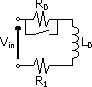
\includegraphics[width=0.25\linewidth]{img/Model_DC_RL_Circuit_General.pdf}
    \caption{Model DC RL Circuit} A DC RL circuit with load $R_0$, inductor $L_0$, resistor $R_1$, and switch for inducing shorts.
    \label{fig:ModelDCRL}
\end{figure}
%\begin{figure}[!htbp]
%	\centering
%    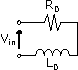
\includegraphics[scale=2.0]{img/DC_RL_Circuit_General.pdf}
%    \caption{An Example DC RL Circuit}
%    \label{fig:DCRL}
%\end{figure}
\subsection{Inductors}
An inductor is a passive electronic component typically illustrated as a coil or four- which resists change in current flow through itself. This property is useful as current through an inductor cannot change instantaneously. Equations describing these properties are provided in Chapter \ref{chap:method of protection}.
\subsubsection{Spatial Parameters}
%Figure of inductor with associated variables. Derivations will be explained later.
The model proposed in Chapter \ref{chap:electronic system model} will rely on a single, air-core inductor. The spatial properties of an inductor may be modeled as seen in Figure \ref{fig:InductorParams}.
\begin{figure}
    \centering
    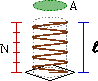
\includegraphics[width=0.25\linewidth]{img/Inductor_Parameters.pdf}
    \caption[Air Core Inductor Spatial Parameters]{Spatial parameters of an air core inductor}
    \label{fig:InductorParams}
\end{figure}
The figure describes a solenoid-style inductor where $N$ represents the number of complete turns, $A$ is the area of a coil, $\ell$ represents the length of the inductor. The relationship between these parameters and inductance can be constructed from fundamental electricity and magnetism equations found in \cite{uniphy}. This relationship is modeled as:
\begin{equation}\label{eq:InductorSpatial}
L = \frac{\mu N^{2}A}{\ell}
\end{equation}
where $\mu$ is the permeability of free space. For our purposes, we assume the spatial parameters are fixed -- i.e., $\ell$, $A$, and $N$ are static\footnote{In Chapter \ref{chap:model optimization}, we consider variable sized inductors as part of our hardware-software co-design optimization.}. Equation (\ref{eq:InductorSpatial}) will be referenced in Chapter \ref{chap:method of protection} to relate current-flow to inductor size and in Chapter \ref{chap:model optimization} to optimize hardware-software co-design solutions.
\subsubsection{Assumption of Constant Turn Density} \label{ssec:Assumption of Constant}
Equation (\ref{eq:InductorSpatial}) contains the term $\frac{N}{\ell}$, referred to as \textit{turn density}. \textit{Turn density} must remain constant with an increase in length for inductance to increase. Thus if an inductor is to be extended from length $\ell$ to $2\cdot \ell$, the number of turns $N$ should be doubled accordingly (to $2\cdot N$) to maintain constant \textit{turn density}. Doubling both $N$ and $\ell$ results in doubled inductance $L$. Whenever a change in inductor length $\ell$ is suggested, we assume the number of turns is doubled as well to maintain constant \textit{turn density}. We rely on this assumption throughout Chapter \ref{chap:model optimization}.
\subsubsection{Inductor Core Composition}
The core of a solenoid-style inductor can be defined as the area within the coiled wire. In practice, many inductors are manufactured with ferromagnetic cores which increase the inductance for the same volume. In our model, we assume this core is empty and contains only air. Equation (\ref{eq:InductorSpatial}) reflects this assumption as it applies only to air-core inductors. We view this assumption as an upper bound on board space consumed since ferromagnetic core inductors provide a greater inductance by volume \cite{NiFe}.

\subsection{Definition of Short and Fault Types}
%Define short in the context of this paper
For the purposes of this model, a short is defined as the flow of current through an alternate, unintended path in a circuit with little or no impedance. In the event of a short, this loss of impedance causes a large change in current which can be slowed and detected through careful reliance on an inductor's ability to resist instantaneous changes in current. However, short-circuits lead to joule heating, the process whereby current through a conductor releases heat modeled as:
\begin{equation}\label{eq:JouleHeating}
\text{Heat} \propto R I^{2} t
\end{equation}
Here, $R$ is resistance, $I$ is current, and $t$ is time \cite{uniphy}. The thermal buildup from joule heating is responsible for the permanent damage that can result from a short and therefore serves as motivation for short-circuit protection. Protection from damage, however, requires catching two short-circuit fault types: the Fault under Load (FUL) and the Hard-Switching Fault (HSF).

\subsubsection{Fault Under Load vs Hard-Switching Fault}
In the context of short-circuit protection, a Fault Under Load is a short-circuit fault where a circuit has an active load at the time of the fault. In this type of fault, the current and impedance are both non-zero. Intuitively, this means the circuit is "on" at the instant the short-circuit occurs. The short forces current to rise, often above desired operating ranges. This fault type, commonly analyzed in IGBTs, has been studied in \cite{scanalysis}.

In contrast, a Hard-Switching Fault is a short-circuit fault where the circuit does not have an active load at the time of the fault \cite{hiSpeedProtection}. In contrast to an FUL, an HSF does not have an initial operating current since there must be a short-circuit path before the circuit is "on".

\subsection{Current as a Function of Time}
In the proposed system, a real-time task must be related to the change in current through an inductor. The following equation will provide such a relationship used Chapter \ref{chap:method of protection}:
\begin{equation}\label{eq:CurrentAtTime}
I(t) = \frac{V}{R}(1-e^{-t \frac{R}{L}})
\end{equation}
where $I(t)$ is current at time $t$, $V$ is a constant voltage to the circuit, $R$ is resistance, and $L$ is inductance.
\clearpage \section{Electronic System Model}\label{chap:electronic system model}
%Define the system model and its components (DC RL Circuit, the OCM)
In the previous chapter, an electronics background was provided as context for our approach. In this chapter, we will define and describe the system model from an electronics perspective. Relying on the provided background, we propose an electronics model with four primary components:
\begin{description}
\item [1.] a DC RL circuit to which software-based short-circuit protection is applicable and board space is consumed by air-core solenoid-style inductor,
\item [2.] an Operating Current Model (OCM) to characterize first-order DC RL circuits,
\item [3.] two short-circuit detection methods for first-order DC RL circuits, and
\item [4.] a real-time sporadic task for short protection.
\end{description}

The short-circuit detection methods will be discussed in Chapter \ref{chap:method of protection} and the real-time model (and its utilization analysis under uniprocessor EDF scheduling) will be discussed in Chapter \ref{chap:real-time system model}.

\subsection{DC RL Short-Circuit Schematic}
Figure \ref{fig:ModelDCRL} is a model DC RL circuit with a switch for simulating a short-circuit. This schematic provides the requirements for the monitored, short-protected circuit: a voltage supply $V_{in}$, circuit load $R_{0}$, inductor $L_{0}$, and the optional, low-value resistor $R_{1}$ used for sensing current. If $R_{1}$ is not used, the resistance through inductor $L_{0}$ may be used to calculate current. Note that the short occurs via the switch around $R_{0}$.
%    \begin{figure}
%    	\centering
%        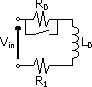
\includegraphics[scale=2.0]{img/Model_DC_RL_Circuit_General.pdf}
%        \caption{A DC RL circuit with load $R_0$, inductor $L_0$, optional resistor $R_1$ and switch for simulating potential shorts.}
%        \label{fig:ModelDCRL}
%    \end{figure}

As previously mentioned, in a manufactured circuit the spatial parameters and inductor value of $L_0$ in Figure \ref{fig:ModelDCRL} are expected to be fixed. During the design phase however, inductor parameters may be altered to increase space efficiency. These properties are afforded by Equation (\ref{eq:InductorSpatial}).

\subsection{Board Space Consumed}
\begin{figure}
    \centering
    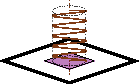
\includegraphics[scale=2.0]{img/Inductor_Perpendicular_Mount.pdf}
    \caption{Board Space Consumed by an Inductor} The highlighted square circumscribing area $A$ of the inductor represents the board space consumed by a solenoid-style air-core inductor.
    \label{fig:BoardSpaceConsumed}
\end{figure}
For ease of analysis, we assume the axis of the inductor is mounted perpendicular to the board as shown in Figure \ref{fig:BoardSpaceConsumed}. Therefore, the board space consumed by the inductor is defined as the square that circumscribes area $A$ of the inductor as seen in Figure \ref{fig:InductorParams}:
\begin{equation}\label{eq:AreaConsumed}
A_{consumed} = \frac{4}{\pi}A
\end{equation}
This definition of board space consumed will be referenced in Chapter \ref{chap:model optimization} where the provided model is optimized for minimum board space consumption and volume.
\subsection{Operating Current Model}
To simplify the analysis of DC RL circuits, we propose an Operating Current Model (OCM) for characterizing the circuit's maximum current, maximum voltage, and critical current. Hereafter, we model DC RL circuits as:
\begin{equation}\label{eq:OCM}
C = (\Gamma_{I}, I_{crit})
\end{equation}
where $C$ is the circuit described using parameters $\Gamma_{I}$ and $I_{crit}$. $\Gamma_{I}$ is defined such that:
\begin{equation}\label{eq:OCMTuples}
\Gamma_{I} = (\gamma_{1},\gamma_{2},...,\gamma_{n})
\end{equation}
\begin{equation}\label{eq:OCMIVPairs}
\gamma_{i} = (I_{i},V_{i})\qquad\text{for all  } i=1,...,n
\end{equation}
Here $\Gamma_{I}$ is composed of $n$ operating current sets $\gamma_{i}$ where $i$ is the index of an operating current set. Each operating current set is a 2-tuple of an operating current, $I_{i}$, and operating voltage, $V_{i}$. The resistance, $R$, of each operating current set can be solved using Ohm's Law and is not included. 

$I_{crit}$ is defined as the critical current of the system as determined by the user. The critical current represents the current value at which the system physically degrades or, in practice, the current value the user wishes to avoid reaching.

Two final derivable parameters $I_{max}$ and $V_{max}$, are extracted from the OCM as follows:
\begin{equation}\label{eq:Imax}
I_{max} = \max_{i \in \Gamma_{I}} \{\gamma_i\} \quad \text{and} \quad V_{max} = \max_{i \in \Gamma_{I}} \{\gamma_i\}
\end{equation}
Note that if $I_{crit} = I_{max}$, any current flow over $I_{max}$ is assumed to be damaging and may not be prevented through this short protection model. Thus, we assume $I_{max} < I_{crit}$.
\clearpage \section{Methods of Protection}\label{chap:method of protection}
%Overview of the methods of short protection.
The intersection of electronics modeling and real-time systems begins with strategies for detecting and halting short-circuits. To detect a short in the generalized first-order DC RL circuit, as seen in Figure \ref{fig:ModelDCRL}, we present two methods for detection:
\begin{description}
\item [1.] a simple comparison of current, $I$, against maximum current, $I_{max}$ and
\item [2.] a comparison of change in current, $\Delta I$, against the maximum change in current, $\Delta I_{\max}$, allowed.
\end{description}
Both methods are applicable to any system which samples current of a monitored circuit. To prevent damage from shorts and fully utilize the following protection methods, power to the monitored circuit(s) must be removed immediately upon detection of a short. Without removal of power, these methods merely support detection and not protection.
\subsection{Method 1: Maximum Operating Current}
The first method for detecting short circuits in a DC RL circuit is to identify when current rises above $I_{max}$. A current value above $I_{max}$ indicates some malfunction caused current to rise above the maximum current in the OCM. When $I > I_{max}$, power to the monitored circuit should be disabled to protect the hardware.
\subsection{Method 2: Maximum Change in Current}
%Define the dI/dt method
The second method of detection requires observing the rate of change of current. From Equation (\ref{eq:CurrentAtTime}) it is known that, given a constant voltage and resistance, the current will converge to $\frac{V}{R}$. During convergence, the slope of $\Delta I$ approaches zero. The derivative of Equation (\ref{eq:CurrentAtTime}) provides the value of $\Delta_{\max}I$:
\begin{equation}
\Delta I = \frac{\partial}{\partial t}I(t) = \frac{\partial}{\partial t}(\frac{V}{R}(1-e^{-t \frac{R}{L}})) = \frac{V}{L}e^{-t \frac{R}{L}}
\end{equation}
Assuming constant inductance, resistance, and voltage, the largest values of $\Delta I$ occur at $t = 0$ and $R = 0$ while excluding infinite inductance ($L \neq +\infty$). This leads to the following conclusions:
\begin{description}
\item [1.] If $R \neq 0$, $\frac{dI(t)}{dt} = \frac{V}{L}$ instantaneously at time $t = 0$ only. Assuming no short has occurred, the change in current between any two consecutive current samples should be less than $\frac{V}{L}$. Formally, $\forall \delta > 0, t \geq 0, \frac{|I(t+\delta) - I(t)|}{\delta} < \frac{V}{L}$ 
\item [2.] If the change in current between two consecutive current samples is equivalent to $\frac{V}{L}$, then $R = 0$ and a short is occurring.
\end{description}

We can safely state the maximum $\Delta I$ through an inductor at any time $t$, including $t = 0$, is:
\begin{equation}\label{eq:DeltaMax}
\Delta_{\max}I = \frac{V}{L} \nonumber
\end{equation}
Since all non-superconducting materials will provide some impedance, the $\Delta_{\max}I$ should have a threshold, $\epsilon$, which serves as an implementation-specific offset. When consecutive current samples are compared, $\Delta_{\max} I = \frac{V}{L} - \epsilon$ should be used as the point of comparison. If a $\Delta I \approx \Delta I_{\max}$, it is likely that $R \approx 0$ and a short is occurring. A benefit of using $\Delta_{\max}I$ is the potential for short detection before $I_{max}$ has been reached. In HSFs, there is no initial current ($I(0) = 0$) which could allow $\Delta I$ to approach $\Delta_{\max}I$ before $I$ exceeds $I_{max}$.
\subsection{Time-to-Detection}
The previous section discussed methods of detecting short-circuits which cover the logical requirements of the real-time short-protection task but did not provide any explicit temporal constraints. As previously mentioned, short-protection systems are time-sensitive and a valuable short-circuit detection occurs before critical current levels are reached. To do so requires determining the time taken for current to rise from its present value, $I$, to the critical current, $I_{crit}$. For the remainder of this paper, we deem this the \textit{time-to-detection}.

\subsubsection{Arbitrary Operating Voltage}
%Define minimum time-to-detection
If the OCM for the circuit in question contains a single operating voltage, it must hold that:
\begin{equation}\label{eq:SingleV}
\forall  V  \in \Gamma_{I}, V = V_{max}
\end{equation}
If Equation (\ref{eq:SingleV}) holds, the \textit{time-to-detection}  is:
\begin{equation}\label{eq:TimeToDetect}
\delta(I,V) = \frac{I_{crit}-I}{V}\cdot L
\end{equation}
where $\delta(I,V)$ is \textit{time-to-detection}, $I$ is current, $I_{crit}$ is the critical current, $V$ is voltage, and $L$ is inductance. The function provides the time required for current to rise from $I$, to the critical current, $I_{crit}$, in a DC RL circuit with voltage $V$ and inductance $L$. This function demonstrates that lower currents and voltages provide a lower \textit{time-to-detection}.
    
However, to use this function for identifying the smallest time-to-detection in an OCM with multiple voltages would be optimistic. Suppose, for example, a DC RL circuit allows for two operating voltages, $V_\ell$ and $V_h$ such that $V_\ell < V_h$. Suppose now that at the instant a short-circuit occurs the operating voltage increases from $V_\ell$ to $V_h$. The value of $\delta(I,V_\ell)$, calculated before the short-circuit ocurred, will be an overestimate of the time required for $I$ to exceed $I_{crit}$. To address this, we define the 

\subsubsection{Maximum Operating Voltage}
Since using Equation (\ref{eq:TimeToDetect}) becomes optimistic when multiple operating voltages are involved, we can remove optimism by replacing $V$ from Equation (\ref{eq:TimeToDetect}) with $V_{max}$:
\begin{equation}\label{eq:TimeToDetectVmax}
\delta(I,V_{max}) = \frac{I_{crit}-I}{V_{max}}\cdot L
\end{equation}
Equation (\ref{eq:TimeToDetectVmax}) ensures a short combined with an instantaneous voltage change to $V_{max}$ is still detected before reaching $I_{crit}$.

\subsubsection{Minimum Time-to-Detection}
%Define minimum time-to-detection
To provide the worst-case time-to-detection, we use the maximum current, $I_{max}$ and voltage, $V_{max}$, from the OCM. This \textit{minimum time-to-detection} is defined as:
\begin{equation}\label{eq:MinTimeToDetect}
\delta_{min} = \delta(I_{max},V_{max}) = \frac{I_{crit}-I_{max}}{V_{max}}\cdot L
\end{equation}
This time frame represents time taken for current to rise from the maximum operating current, $I_{max}$, to the critical current, $I_{crit}$, with the highest voltage, $V_{max}$. This \textit{minimum time-to-detection} will be used as a temporal constraint for the proposed real-time task.
\clearpage \section{Real-time System Model}\label{chap:real-time system model}
%Overview of real-time systems.
Thus far, the spatial properties of an inductor have been related to its inductance. Thereafter, inductance is found to determine the maximum possible current rise at any given time, $\frac{V}{L}$ Amperes per second. This leads to the shortest time span over which a short would need to be detected, the \textit{minimum time-to-detection} $\delta_{min}$. Using $\delta_{min}$, we provide a real-time system short-circuit protection task and its timing requirements. Before doing so, we present a real-time background on the sporadic task model and uniprocessor EDF scheduling.

\subsection{Sporadic Task Model}
In real-time systems, \textit{sporadic tasks} are defined by a \textit{worst-case execution time} (WCET) $e_{i}$, relative deadline $d_{i}$, and minimum period $p_{i}$. The relative deadline is the time between each job arrival and its deadline. The minimum period is the smallest time between successive job arrivals. We use a sporadic task to model the short-circuit protection task \cite{sporadicTaskModel}. The proposed sporadic task will have an \textit{implicit deadline} where a new job of the short-circuit task $\mathrm{T}_{scd}$ may arrive at the absolute deadline of the previous job.

For our short-circuit task $\mathrm{T}_{scd}$, the execution time depends on the short-circuit protection algorithm used, processor speed, and ADC conversion time. Thus, the execution time is not assessed here but modeled as $e_{scd}$.

The minimum period, however, is derived from Equation (\ref{eq:TimeToDetectVmax}) which provides a scaling \textit{time-to-detection}. The minimum period of the sporadic task must be half the value of the \textit{minimum time-to-detection}. This is required to ensure one full job of $\mathrm{T}_{scd}$ is completed strictly after the short-circuit begins. This requirement is demonstrated in Figures \ref{fig:shortedschedule} and \ref{fig:stoppedschedule} where $\mathrm{T}_{scd}$ executes with a period equal to $\delta_{min}$ and $\frac{\delta_{min}}{2}$. Recall that $\delta_{min}$ time units after a short, the current level has reached a $I_{crit}$. Each sporadic job is triggered $\delta(I,V_{max})/2$ seconds after the release of the preceding job, allowing release times to scale with current. The temporal requirements may be converted into a real-time sporadic task $\mathrm{T}_{scd} = (e_{scd}, p_{scd})$ with the following parameters:
\begin{equation}\label{eq:ExecutionTime}
e_{scd} = \textit{worst case execution time }\text{of short-circuit algorithm}
\end{equation}
\begin{equation}\label{eq:Period}
p_{scd} = \frac{\delta(I_{max},V_{max})}{2}
\end{equation}
\begin{figure}
    \centering
    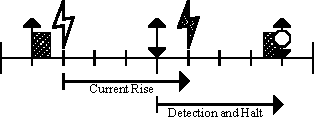
\includegraphics[width=0.60\linewidth]{img/shortedschedule.pdf}
    \caption{Failed Short Protection Schedule} $\mathrm{T}_{scd}$ executing with $p_{scd} = \delta(I_{max},V_{max}) = 4$.\\The short begins at $t = 2$ and $I_{crit}$ is reached at $t = 6$ before $\mathrm{T}_{scd}$ can halt the short.
    \label{fig:shortedschedule}
\end{figure}
\begin{figure}
    \centering
    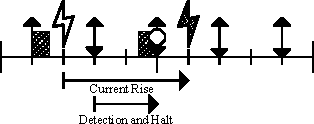
\includegraphics[width=0.60\linewidth]{img/stoppedschedule.pdf}
    \caption{Successful Short Protection Schedule} $\mathrm{T}_{scd}$ executing with $p_{scd} = \frac{\delta(I_{max},V_{max})}{2} = 2$.\\The short begins at $t = 2$ and is halted by $\mathrm{T}_{scd}$ at $t = 5$ before $I_{crit}$ is reached.
    \label{fig:stoppedschedule}
\end{figure}
%Game Fucking Over
\subsection{Preemptive Uniprocessor EDF Scheduling}
%Cite optimality of uniprocessor preemptive EDF scheduling
%Cite utilization calculation for uniprocessor preemptive EDF scheduling.
With $\mathrm{T}_{scd}$ defined, we derive its utilization under preemptive uniprocessor EDF scheduling. According to \cite{LiuLayland}, a set of implicit-deadline sporadic tasks is schedulable with EDF if and only if:
\begin{equation}\label{eq:EDFUtilization}
\sum_{i=1}^{n} \frac{e_{i}}{p_{i}} \leq 1
\end{equation}
where $i$ is the index of a task in the set, $e_{i}$ is the execution time, and $p_{i}$ is the period. Since we use a single, sporadic task with implicit deadlines, the utilization for $\mathrm{T}_{scd}$ is:
\begin{equation}\label{eq:SCDUtilization}
U(\mathrm{T}_{scd}) = \frac{2 \cdot e_{scd}}{\delta(I,V_{max})}
\end{equation}
Using the \textit{minimum time-to-detection}, Equation (\ref{eq:SCDUtilization}) becomes:
\begin{equation}\label{eq:SCDMinUtilization}
U(\mathrm{T}_{scd}) = \frac{2 \cdot e_{scd}}{\delta(I_{max},V_{max})}
\end{equation}
Substituting in Equations (\ref{eq:TimeToDetect}) and (\ref{eq:InductorSpatial}) gives:
\begin{equation}\label{eq:SCDSpatialUtilization}
U(\mathrm{T}_{scd}) = (\frac{2 \cdot e_{scd}}{(I_{crit}-I_{max})} \cdot V_{max} \cdot \frac{\ell}{\mu N^{2}A})
\end{equation}
Equation \ref{eq:SCDSpatialUtilization} relates the inductor spatial parameters to $\mathrm{T}_{scd}$ utilization.

%\subsection{Detection as a Hard Real-Time Task}
%As previously mentioned, the correctness of a real-time computation has a temporal component, in this case the relative deadline. A real-time task in which %results produced after a deadline have some utility is a \textit{soft} real-time task. Video rendering could be considered a soft real-time task. One in which %a result produced after a deadline has no utility but results in no damage is considered \textit{firm}. In the case of the proposed real-time task, results %produced after a deadline may cause have disastrous consequences including damage to the controlled system \cite{rts}.
%\clearpage \section{Real-time Utilization Requirement for Short Detection}

\clearpage \section{Model Optimization}\label{chap:model optimization}
Having related the board space consumed by an inductor and the real-time utilization under EDF schedulability, we propose an optimal solution for fixed values on either end of the relationship. Given a fixed utilization we propose a minimized board space consumption. Given a fixed allowable board space, we propose a minimized real-time utilization. Before optimization analysis of the model, we clarify the optimal inductor orientation for a given prism.

\subsection{Optimal Inductor Orientation}
In practice, hardware-software co-design is constrained by real-world factors such as size, weight, power, and cost. In this paper, we focus on space as a constraint on our proposed model.
Given a fixed volume of space to implement the proposed short-protection system, we must consider the optimal orientation of our solenoid-style air-core inductor inside the fixed volume which maximizes inductance. 
To find the inductor orientation providing the highest inductance for a given space, we consider two constraints:
\begin{description}
\item [1.] The area $A$ from Equation (\ref{eq:InductorSpatial}) requires a square area with regard to board space.
\item [2.] The board space must be defined in three dimensions: a length $\ell$, width $w$, and height $h$.
\end{description}
Allowable board space is therefore defined as a set:
\begin{equation}\label{eq:Prism}
P = \{\ell,w,h\}
\end{equation}
This set provides the prism dimensions in which the inductor resides. Independent of the prism's orientation, $A_{consumed}$ must be the smallest square to circumscribe the area $A$ of the inductor. The largest square face on which the inductor's area, $A$, can be placed is limited by the median dimension in P. Thus, the square of the median is used to fit the largest possible square area:
\begin{equation}\label{eq:PrismAreaConsumed}
A_{consumed} = median(P)^2
\end{equation}
The only remaining dimension is deemed the length of the inductor:
\begin{equation}\label{eq:PrismLength}
\ell = min(P)
\end{equation}

A visualization of possible orientations can be found in Appendix \ref{appendix:orientation-visualization} along with an explicit example. As previously mentioned and validated in Section \ref{ssec:Assumption of Constant}, the \textit{Assumption of Constant Turn Density} applies to $\ell$ and is required for the remaining model optimization.


\subsection{Fixed Board Constraints}

Having defined equations for consumed area in terms of the volume allotted for the inductor, we address the first optimization problem where the board space is constrained. This approach is useful in situations where the embedded application, or the region of space allotted for short-circuit protection hardware, is restricted in size. Suppose allotted board space is restricted to the prism:
\begin{equation}\label{eq:Prism2}
P = \{\ell, w, h\} \nonumber
\end{equation}
where each element of the set is defined in meters. Combining Equations (\ref{eq:AreaConsumed}) and (\ref{eq:PrismAreaConsumed}) for the area of the inductor $A$ gives:
\begin{equation}\label{eq:InductorAreaPrism}
A = \frac{\pi}{4} A_{consumed} = \frac{\pi}{4} \cdot median(P)^2 \nonumber
\end{equation}
By substitution of Equation \ref{eq:InductorAreaPrism} into Equation (\ref{eq:SCDSpatialUtilization}), the utilization requirement becomes:
\begin{equation}\label{eq:MinUtilizationPrism}
U(\mathrm{T}_{scd}) = \frac{2 \cdot e_{scd} \cdot V_{max} \cdot min(P)}{(I_{crit}-I_{max}) \cdot \mu \cdot N^{2} \cdot \frac{\pi}{4} \cdot median(P)^2}
\end{equation}
The equation above gives us a minimum utilization requirement for meeting short-circuit protection requirements given the constrained board space and OCM - which provides $I_{crit}$ and $I_{max}$.

\subsection{Fixed Utilization}
Having addressed the fixed-volume constraint, we not address the second approach by fixing the maximum utilization allowed short-circuit protection process.
This approach is useful in situations where the microprocessor executing $\mathrm{T}_{scd}$ is responsible for other tasks which inherently limit $U(\mathrm{T_{scd}})$. Suppose the allotted utilization is $u$. Relying on Equation (\ref{eq:SCDMinUtilization}) we find the minimum time-to-detection $\delta(I_{max},V_{max})$ is solved as:
\begin{equation}\label{eq:MinTimeToDetectSpatial}
\delta_{min} = \delta(I_{max},V_{max}) = \frac{2 \cdot e_{scd}}{u} \nonumber
\end{equation}
Applying Equation (\ref{eq:MinTimeToDetect}) and isolating $L$ we find:
\begin{equation}\label{eq:InductorFixedUtilization}
L = \frac{2 \cdot e_{scd} \cdot V_{max}}{u \cdot (I_{crit}-I_{max})} \nonumber
\end{equation}
Substituting Equation (\ref{eq:InductorSpatial}) in for $L$ 
%gives:
%\begin{equation}\label{eq:MinPrismUtilizationUnsolved}
%\frac{\mu N^{2}A}{\ell} = \frac{2 \cdot e_{scd} \cdot V_{max}}{u \cdot (I_{crit}-I_{max})} \nonumber
%\end{equation}
and isolating inductor spatial parameters results in:
\begin{equation}\label{eq:MinPrismUtilizationUnsolved2}
\frac{A}{\ell} = \frac{2 \cdot e_{scd} \cdot V_{max}}{u \cdot (I_{crit}-I_{max}) \cdot \mu \cdot N^{2}} \nonumber
\end{equation}
Finally, substituting the prism area consumed (Equation \ref{eq:PrismAreaConsumed}) and prism length (Equation \ref{eq:PrismLength}) into Equation \ref{eq:MinPrismUtilizationUnsolved2} above gives:
\begin{equation}\label{eq:MinPrismUtilization}
\frac{median(P)^{2}}{min(P)} = \frac{4}{\pi} \cdot \frac{ 2 \cdot e_{scd} \cdot V_{max}}{u \cdot (I_{crit}-I_{max}) \cdot \mu \cdot N^{2}}
\end{equation}
This result indicates the air core inductor used in the DC RL circuit must have a minimum allotted board space defined by P which satisfies the above equation.

The model optimizations above highlight how fixed board space can be used to prescribe a minimum utilization and vice versa. We now seek to validate our short-circuit protection model the next chapter where we discuss our experiments and subsequently our results.

\clearpage \section{Experiments}\label{chap:experiments}
To implement and validate the application of the software-based approach, we conducted four separate experiments. The following section presents the experiment setup and outlines the conducted experiments. Additionally, the projected utilization for the experiments is presented.

\subsection{Experiment Outline}
The experiments conducted measured both FUL and HSF short-circuits focusing primarily on FUL short-circuits as they have a smaller time-to-detection.
Table \ref{tab:ExperimentDescriptions} highlights the variations between experiments which can be summarized as follows:
Experiment 1 examines the performance of our approach under FUL short-circuits in terms of detection latency and maximum current reached at the time of detection. Experiment 2 examines the performance under HSF short-circuits also in terms of latency and maximum current reached at the time of detection.
Experiment 3 demonstrates how fixing utilization and varying inductance under FUL short-circuits relates to current at the time of detection.
Experiment 4 demonstrates the same relationship but with varying utilization and fixed inductance.
\begin{table}[!h]
    \centering	
    \bgroup
    \def\arraystretch{1.00}%  1 is the default, change whatever you need
    \begin{tabular}{| c | c | c | c |}
            \hline			
            Experiment & Fault Type & Demonstrates\\ \hline \hline \cline{1-3}
            1 & FUL & Baseline\\ \hline
            2 & HSF & Lower initial $I$\\ \hline
            3 & FUL & Scaling $L$\\ \hline
            4 & FUL & Scaling $U$\\ \hline  
    \end{tabular}
    \egroup
    \caption{Experiment Descriptions}
    \label{tab:ExperimentDescriptions}
\end{table}

\subsection{Setup}
Aside from the variations described above, all experiments were conducted as described here. Short-circuit protection for each experiment was performed on Microchip's DM164103-4 demo board with a PIC18F45K20 CPU. The demo board and programmer were selected for their relatively low cost to encourage reproducibility. 
Figure \ref{fig:ExperimentSetup} depicts the experimental circuit schematic. In the schematic, subscripts \textit{DM} refer to connections made to the Microchip demo board. The setup also requires attaching oscilloscope probes to ports RA2 in Figure \ref{fig:ExperimentSetup} and RA1 on the demo board. Figure \ref{fig:Experiment1Setup} depicts the proper connection of all materials in Experiment 1. All probe connections route off-camera to the oscilloscope. An extended list of non-trivial materials used in the experiments can be found in Appendix \ref{appendix:materials}.
\begin{figure}
    \centering
    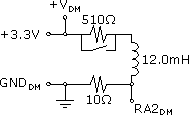
\includegraphics[width=0.45\linewidth]{img/Experiment_Setup.pdf}
    \caption{Experiment Setup Schematic} Experiment Setup Schematic
    \label{fig:ExperimentSetup}
\end{figure}

\begin{figure}
    \centering
    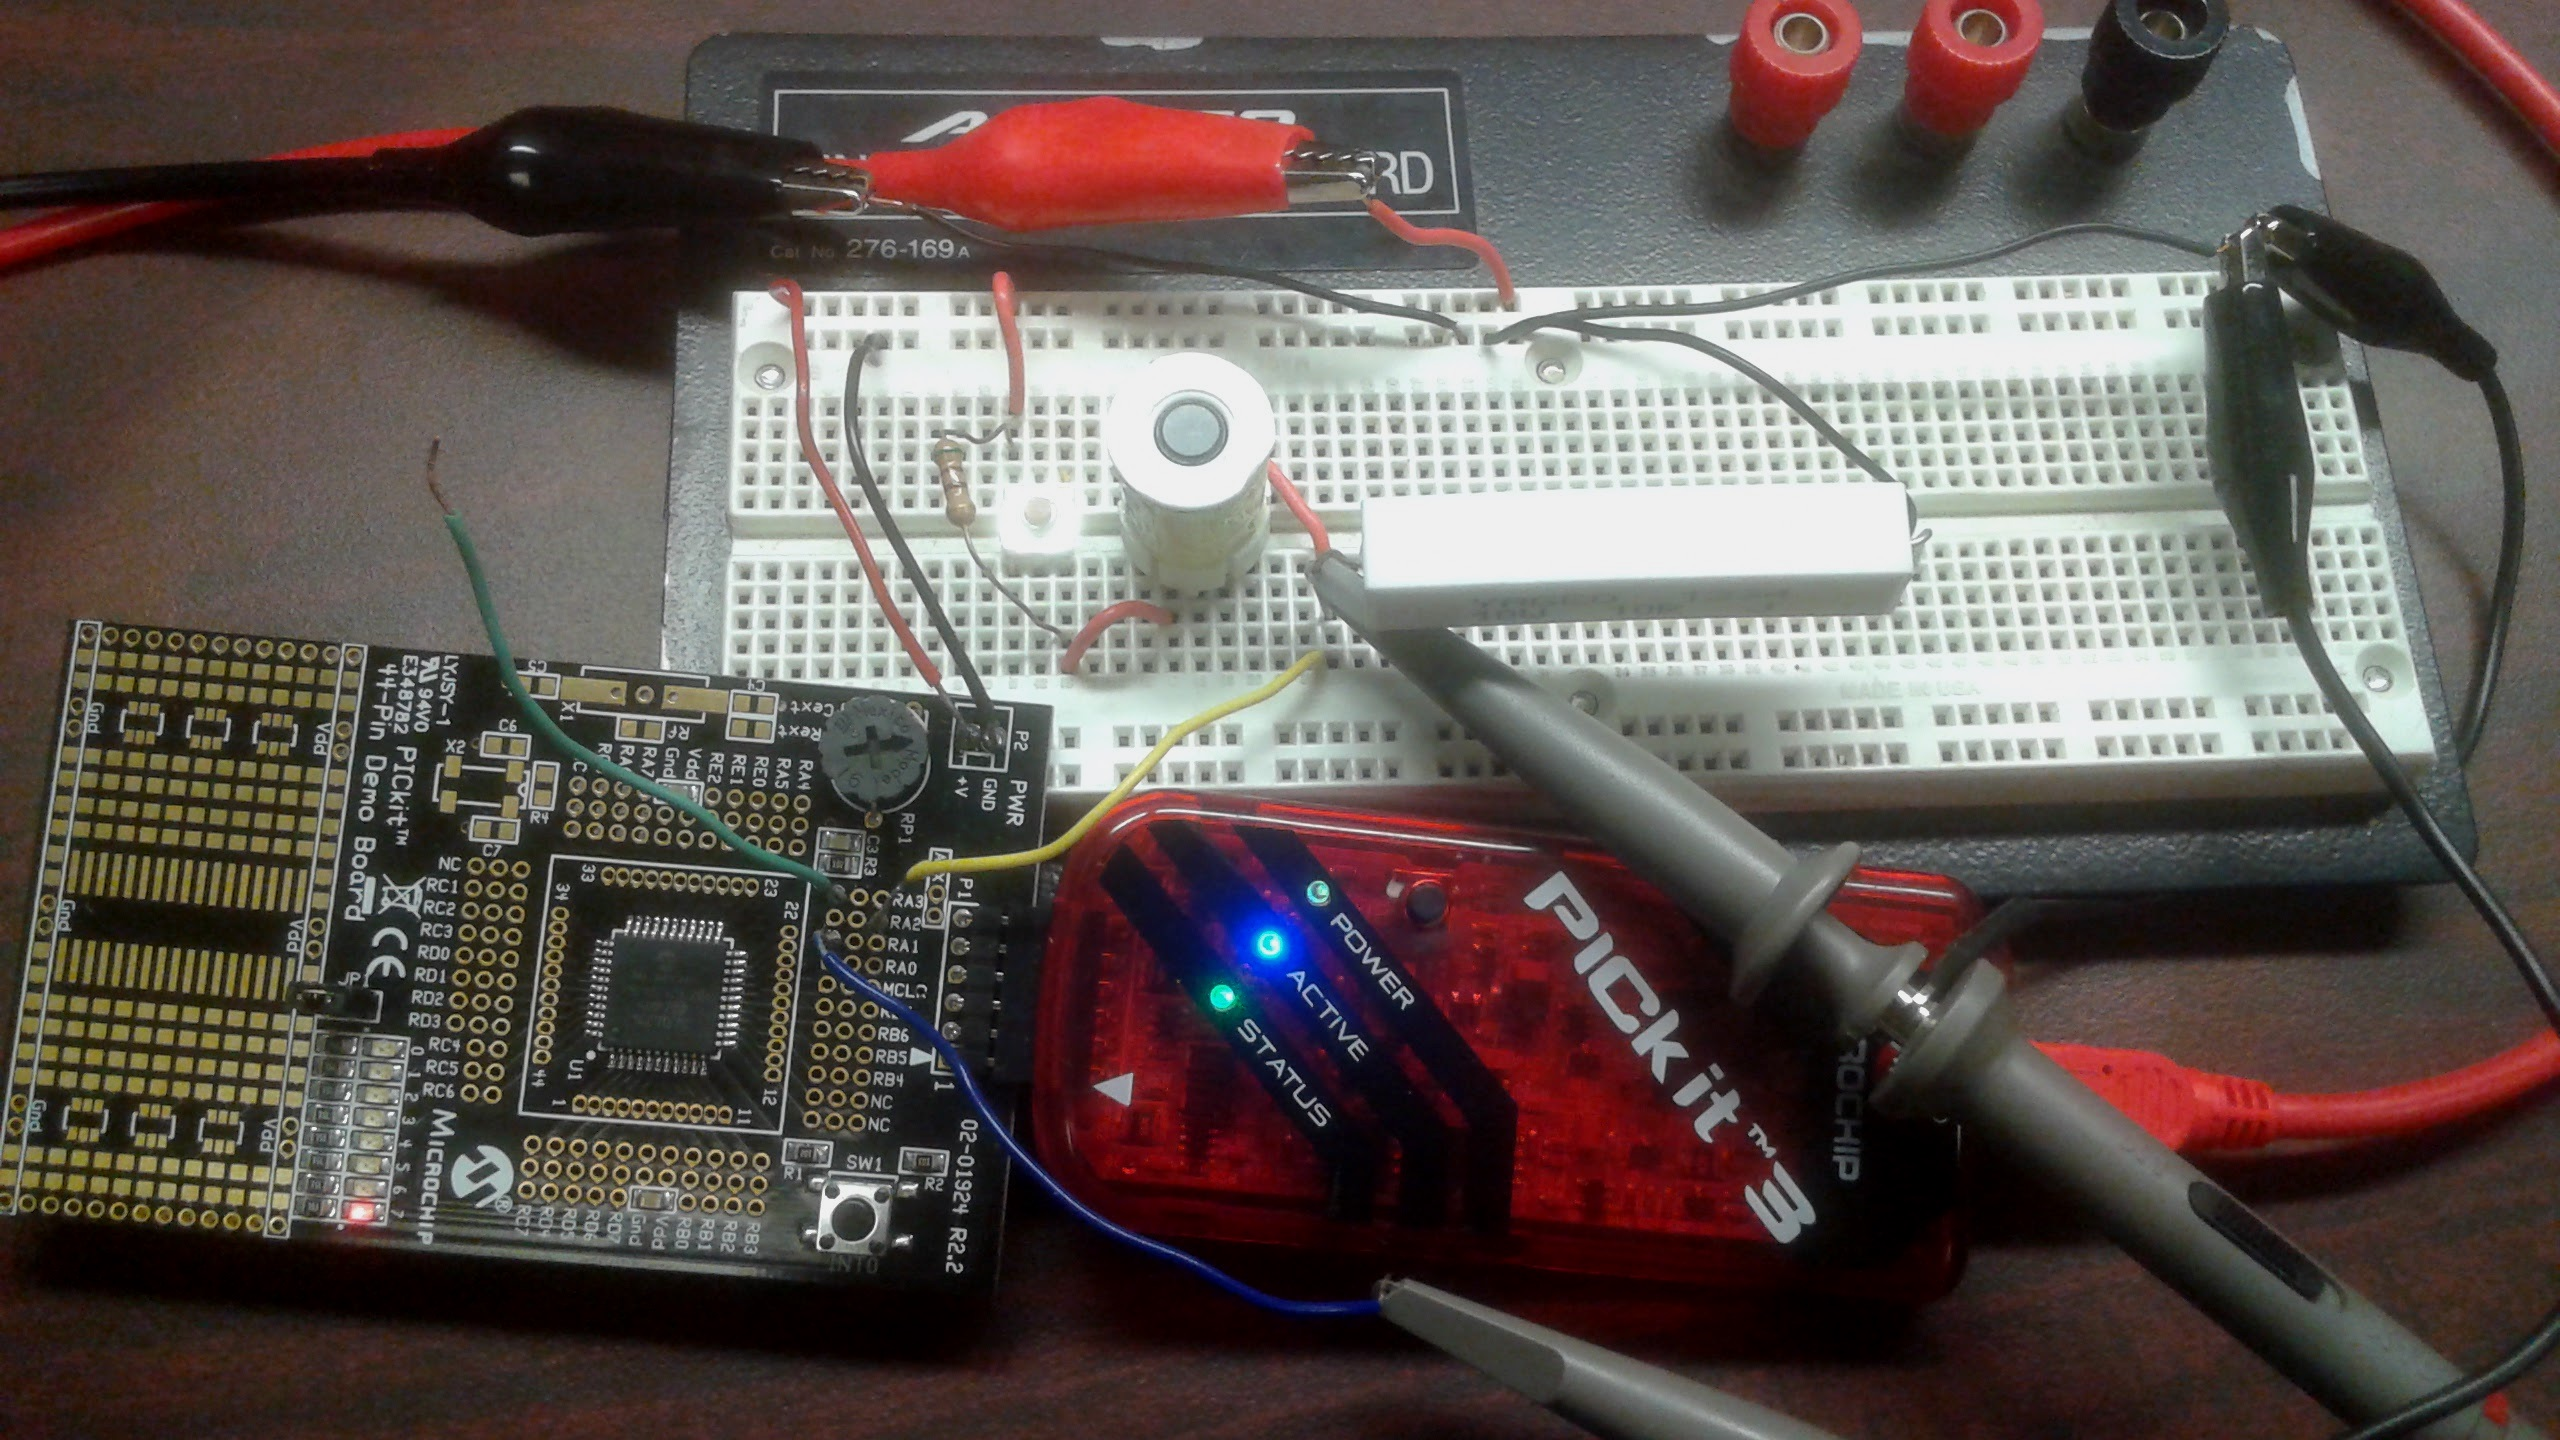
\includegraphics[width=0.75\linewidth]{img/SCD_5_9mH_EXP_SETUP.jpg}
    \caption{Experiment Setup Image}
    \label{fig:Experiment1Setup}
\end{figure}

The circuit was run in advance of experiments to identify experimental operating currents and voltages and their respective maximums. This process could be avoided by analyzing the tolerance values for all components used but was explicitly measured here to provide exact values. The OCM for the setup using solid, 22 American Wire Gauge (AWG) copper wire was:
\begin{equation}\label{eq:OCMSetup}
C = (\Gamma_{I}, 150mA) \quad \Gamma_{I} = (\gamma_{0}) \quad \gamma_{0} = (7.74mA, 3.3V) \nonumber
\end{equation}

Although the resistor $R_{1}$ pictured in \ref{fig:Experiment1Setup} is a 10W power resistor capable of handling higher current, we defer to the power rating of a conventional though-hole power resistor which we assume to be 0.5 Watts. Since 150 mA through a 0.5 Watt resistor exceeds the power rating at an operating voltage of 3.3 V, 150 mA is considered the critical current $I_{crit}$ for the circuit.

After deriving the OCM from the circuit, Equation (\ref{eq:Imax}) provides the maximum operating current and voltage:
\begin{equation}
I_{max} =  7.74mA \nonumber \quad V_{max} = 3.3V \nonumber
\end{equation}
Note that the critical current is 150mA meaning current above 7.74mA is considered unexpected behavior while current at or above 150mA is damaging. Having constructed the mathematical model of our system, we may now project the utilization requirement in the following section. 

%TODO - Delete?
%Using the OCM, values for $I_{max}$ and $\Delta_{\max}I$ can be converted to the appropriate ADC values.
%Conversion of the ADC resolution to $\frac{\text{Volts}}{\text{ADC Tick}}$ is left to the reader as it is system-dependent. The resolution is then used to convert $I_{max}$ and $\Delta I$ to ADC values.
\subsection{Projected Utilization}
Using the OCM derived from the experiment setup, we apply Equations \ref{eq:SCDUtilization} and \ref{eq:SCDMinUtilization} as the scaling utilization and minimum utilization. For this projected utilization, our protection method required an execution time of 25 microseconds. Figure \ref{fig:Simulated Utilization} depicts the projection of fixed minimum utilization and the scaling utilization. The minimum utilization indicates the expected minimum utilization required to detect a short-circuit in the experiment. The scaling utilization represents the minimum utilization required at \textit{any} given value of $I$ as derived from Equation (\ref{eq:SCDUtilization}). These projected utilizations indicate the provided short-protection approach could safely detect and halt a short-circuit before critical current levels are reached at a uniprocessor utilization of under 0.1. The scaling utilization curve indicates the lower minimum utilization requirement for systems with lower operating currents.

\begin{figure}
\centering
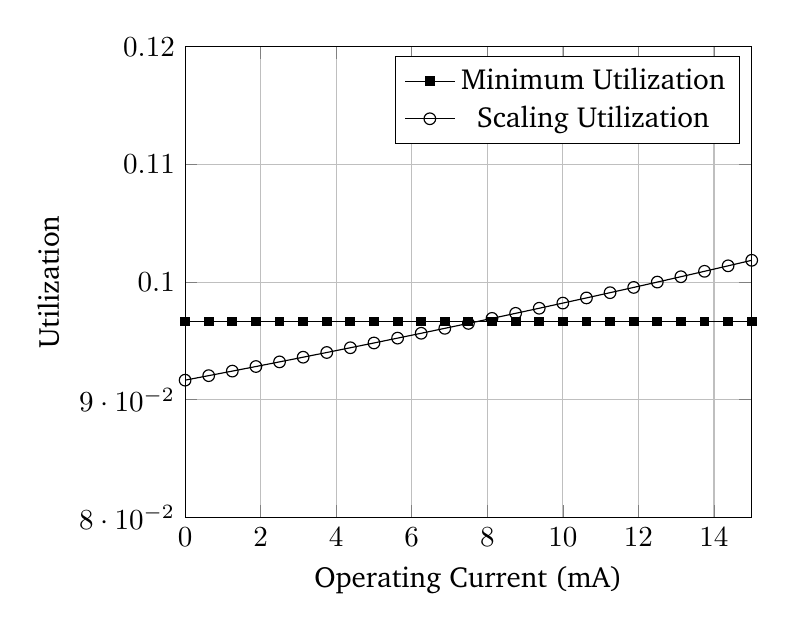
\begin{tikzpicture}[scale=1.05]
    \begin{axis}[ 
    xlabel=Operating Current (mA),
    ylabel=Utilization,
    grid=major,
    xmin=0.00,xmax=15.0,
    ymin=0.08,ymax=0.12
        ] 
    \addplot [mark size=1.5, mark=square*, domain=0:15, samples=25]{(2*0.000025*3.3)/(0.0120*(150 - 7.74))*1000};
    \addplot [mark size=2.0, mark=o, domain=0:15, samples=25]{(2*0.000025*3.3)/(0.0120*(150 - x))*1000};
    \legend{Minimum Utilization,Scaling Utilization}
    \end{axis}
\end{tikzpicture}
    \caption{Simulated Utilization vs. Operating Current}
    \label{fig:Simulated Utilization}
\end{figure}

\clearpage \section{Results}\label{chap:results}
\subsection{Experiments 1 and 2: FUL and HSF Detection}
To validate the hardware-software co-design approach, two short-circuit fault types were induced in separate experiments. As shown in Table \ref{tab:ExperimentDescriptions}, Experiment 1 induced an FUL short while Experiment 2 inducted an HSF short. Each experiment was run three times with all data provided in Table \ref{tab:FULHSFComparison}. In the table, $I_{c}$ is the current at the time of detection and $\Delta t$ is the latency between short-circuit and detection. Three runs per fault type was selected due to time required to manually induce the short and reset each experiment.

\begin{table}
    \centering
    \bgroup
    \def\arraystretch{1.25}%  1 is the default, change whatever you need
    \begin{tabular}{| c | c | c | c | c |}
            \hline			
            Fault & R (Ohm) & $I_{c}$ (mA) & $\Delta t$ (us) & U($\mathrm{T}_{scd}$)\\ \hline \hline \cline{1-5}
%  		FUL & 510 & 31.867 & 132.27 & 0.1316\\  \hline %Original Averages
%  		HSF &   0 & 33.733 & 117.59 & 0.1316\\  \hline %Original Averages
        FUL & 510 & 42.400 & 159.79 & 0.1316\\ \hline
        FUL & 510 & 38.800 & 142.59 & 0.1316\\	\hline
        FUL & 510 & 20.000 &  50.39 & 0.1316\\	\hline
        HSF &   0 & 35.200 & 149.60 & 0.1316\\	\hline
        HSF &   0 & 35.200 &  72.01 & 0.1316\\	\hline
        HSF &   0 & 35.200 & 175.20 & 0.1316\\	\hline
        \end{tabular}
    \egroup
    \caption{FUL and HSF Comparison}
    \label{tab:FULHSFComparison}
\end{table}

Both experiments demonstrate successful detection of FUL and HSF short-circuits before current rises above $I_{crit}$. Both experiments also demonstrate latency one-tenth of the minimum time to detection. For experiment 1, using the FUL, the short-circuit was manually induced while the circuit was powered. In contrast, experiment 2 required removal of load resistor $R_{0}$ from Figure \ref{fig:ExperimentSetup}. This ensures the short-circuit begins immediately upon powering the circuit. As a result of this change, there is no initial current in the HSF as there is with the FUL short.

In addition to the comparison table, an example FUL waveform is shown in Figure \ref{fig:FULShort} as it was the most used short-circuit fault test. The plot shows the circuit current, sampled on port RA2, rise immediately after the short-circuit. The short-circuit detection signal, output on port RA1, shows the output signal voltage drop to zero indicating the detection of a fault and the cutting of power by the microprocessor. Due to its similar nature, the waveform for the HSF experiment is excluded. The current at the time of detection for both fault types in all runs did not exceed $I_{crit}$, 150mA; thus, the proposed short-circuit protection succeeded in safely mitigating damage from both FUL and HSF short-circuits.

\begin{figure}
    \centering
    \begin{tikzpicture}[scale=0.90]
    \begin{axis}[
        grid=major,
        axis y line*=left,
        xlabel=Time (s),
        ylabel=RA2 (V)]
    \addplot[mark size=0.07, mark=o, red, each nth point={10}] table [x=Time, y=RA2, col sep=comma] {data/rawdata/ECRTS17data/fc.csv};
    \label{RAplot}
    \addlegendentry{$RA2$};
    \end{axis}
    \begin{axis}[
        ylabel near ticks, yticklabel pos=right,
        axis x line=none,
        ylabel=RA1 (V)]
        \addlegendimage{/pgfplots/refstyle=RAplot}
        \addlegendentry{$RA2$}
    \addplot[mark size=0.7, mark=square*, blue, each nth point={100}] table [x=Time, y=RA1, col sep=comma] {data/rawdata/ECRTS17data/fc.csv};
    \addlegendentry{$RA1$};
    \draw[mark=square*] (axis cs:\pgfkeysvalueof{/pgfplots/xmin},1.96000e-01) -- (axis cs:\pgfkeysvalueof{/pgfplots/xmax},1.96000e-01);
    \end{axis}
    \end{tikzpicture}
    \caption{FUL Short Waveform}
    \label{fig:FULShort}
\end{figure}

\subsection{Experiments 3 and 4: Inductance and Utilization Scaling}
Experiments 3 and 4 focused on demonstrating the potential for scaling inductance and utilization as co-design parameters are changed.
In Experiment 3, the schematic depicted in Figure \ref{fig:ExperimentSetup} was used with varying sized inductors as opposed to experiment 1 and 2 which used fixed values. For each inductance value, $L$, a FUL short was induced. Real-time utilization was maximized at 100\%, $U = 1.0$, to demonstrate the broadest range of inductors. As seen in Figure \ref{fig:ScalingInductance}, a decrease in inductance given a constant utilization results in a higher current at the time of detection. This trend validates the relationship presented in Equation \ref{eq:SCDSpatialUtilization}. In conjunction with the optimal inductor orientation analysis, the results show short-circuit detection at lower current levels can be traded for a smaller inductor consuming less board space.

A similar procedure was used in Experiment 4 but with fixed inductor sizes and varying real-time utilizations. In Experiment 4, the schematic in Figure \ref{fig:ExperimentSetup} is used but with an inductance of $L = 12 \text{mh}$.  This large value of inductance was selected to demonstrate the broadest range of real-time utilizations. The results, presented in Figure \ref{fig:ScalingUtilization}, show a decrease in utilization given a constant inductance leads to a higher current at the time of detection. This again validates the relationship provided in Equation (\ref{eq:SCDSpatialUtilization}).

The results of Experiment 3 and Experiment 4 indicate that $U(\mathrm{T}_{scd})$ can be traded with inductance $L$ in our model to maintain a stable current at the time of detection. It follows that inductor size and board space consumed by the proposed short-circuit protection model may be traded with the utilization of the provided software-based protection approach.

\begin{figure}
    \centering
    \begin{tikzpicture}[scale=1.00]
    \begin{axis}[
            grid=major,
        xlabel=Current at Detection (mA),
        ylabel=Inductance (H)]
    %\addplot[no markers] table [ col sep=comma, x=Ic, y={create col/linear regression={y=Inductance, x=Ic}}] {data/aggregate/exp3runs.csv};
    \addplot[only marks, mark=square*, mark size=3.5] table [x=Ic_mA, y=L, col sep=comma] {data/aggregate/ECRTS17data/L120.csv};
    \addplot[only marks, mark=x, mark size=5.0] table [x=Ic_mA, y=L, col sep=comma] {data/aggregate/ECRTS17data/L095.csv};
    \addplot[only marks, mark=*, mark size=3.0] table [x=Ic_mA, y=L, col sep=comma] {data/aggregate/ECRTS17data/L081.csv};
    \addplot[only marks, mark=triangle*, mark size=3.0] table [x=Ic_mA, y=L, col sep=comma] {data/aggregate/ECRTS17data/L056.csv};
    \addplot[only marks, mark=o, mark size=3.0] table [x=Ic_mA, y=L, col sep=comma] {data/aggregate/ECRTS17data/L039.csv};
    \legend{$L=12.0mH$,$L=9.5mH$,$L=8.1mH$,$L=5.6mH$,$L=3.9mH$}
    \end{axis}
    \end{tikzpicture}
    \caption{Experiment 3 Results: Scaling Inductance vs Current at Detection}
    \label{fig:ScalingInductance}
\end{figure}
\begin{figure}
    \centering
    \begin{tikzpicture}[scale=1.00]
    \begin{axis}[
        grid=major,
        xlabel=Current at Detection (mA),
        ylabel=Utilization]
    %\addplot[no markers] table [ col sep=comma, x=Ic, y={create col/linear regression={y=Utilization, x=Ic}}] {data/aggregate/exp4runs.csv};
    \addplot[only marks, mark=square*, mark size=3.5] table [x=Ic_mA, y=U, col sep=comma] {data/aggregate/ECRTS17data/U1000.csv};
    \addplot[only marks, mark=x, mark size=5.0] table [x=Ic_mA, y=U, col sep=comma] {data/aggregate/ECRTS17data/U0694.csv};
    \addplot[only marks, mark=*, mark size=3.0] table [x=Ic_mA, y=U, col sep=comma] {data/aggregate/ECRTS17data/U0500.csv};
    \addplot[only marks, mark=triangle*, mark size=3.0] table [x=Ic_mA, y=U, col sep=comma] {data/aggregate/ECRTS17data/U0250.csv};
    \addplot[only marks, mark=o, mark size=3.0] table [x=Ic_mA, y=U, col sep=comma] {data/aggregate/ECRTS17data/U0130.csv};
    \legend{$U=1.0000$,$U=0.694$,$U=0.5000$,$U=0.2500$,$U=0.1316$}
    \end{axis}
    \end{tikzpicture}
        \caption{Experiment 4 Results: Scaling Utilization vs Current at Detection}
    \label{fig:ScalingUtilization}
\end{figure}

\clearpage \section{Conclusion} \label{chap:conclusion}
%The conclusion goes here: use hypothesis from proposal as basis
This work provides a novel solution for hardware-software co-design of real-time software-based short-circuit protection systems -- cyber-physical systems in which the inductive properties of a DC RL circuit are leveraged to construct a sporadic, real-time short-circuit protection task. We established a relationship between utilization and board space consumed by the air-core, solenoid-style inductor placed in-circuit which can be optimized for both fixed inductor volume and fixed uniprocessor utilization.

Like preceding works on engine control \cite{engineCtrl} and thermal-aware systems \cite{thermalAware}, this work demands further investigation into the real-time control of physical systems demonstrating dynamic behavior. Further study on the energy and performance trade-off between hardware, software, and physical system dynamics is reserved for future work.

\clearpage
\centerline{\large\bf APPENDIX A}
\addcontentsline{toc}{section}{Appendix A}
\appendix{Materials}\label{appendix:materials}
Non-trivial materials used in the experiments can be found in Figure \ref{fig:Materials}. Excluded from the materials list are elements including cooper wire, breadboards, and a power supply. To minimize cost of replication, through-hole parts are used in place of smaller, surface-mount components.
\begin{figure}[!htbp]
    \centering	
    \bgroup
    \def\arraystretch{1.25}%  1 is the default, change whatever you need
    \begin{tabular}{| c | c | c |}
        \hline			
        Item & Manufacturer & Part Number(s)\\ \hline \hline \cline{1-3}
        Debugger & Microchip & PG164130\\ \hline
        Inductor & Triad Magnetics & RC-1; RC-2; RC-3\\ \hline
        Microprocessor & Microchip & DM164130-4\\ \hline
        Oscilloscope & RIGOL & DS1102E\\ \hline
        Oscilloscope Probe & HANTEK & PP-150\\  \hline  
        Power Resistor & YAGEO & 1334 10W 10R J\\  \hline  
        Resistor & N/A & 510$\Omega$ 5\% resistor\\  \hline  
    \end{tabular}
    \egroup
    \caption{Materials List}Materials list for Experiments 1-4
    \label{fig:Materials}
\end{figure}

\clearpage
\centerline{\large\bf APPENDIX B}
\addcontentsline{toc}{section}{Appendix B}

\appendix{Inductor Orientation Visualization}\label{appendix:orientation-visualization}
Given an allowable board space defined as a prism, $P = \{\ell, w, h\}$, there are only three unique orientations for an air-core, solenoid-style inductor in the space. The inductor may be oriented with $A$ located on:
\begin{description}
\item[1.] the plane formed by $l$ and $w$ extending along $h$.
\item[2.] the plane formed by $l$ and $h$ extending along $w$.
\item[3.] the plane formed by $w$ and $h$ extending along $l$.
\end{description}

Figure \ref{fig:PossibleOrientations} depicts each of these orientations inside a prism with dimensions:

\begin{equation}\label{eq:PrismSimulation}
P = \{3, 2, 1\} \nonumber
\end{equation}

Notice the inductor consuming the most volume has its area $A$ on the plane formed by the two largest dimensions.

\begin{figure}[!htbp]
    \centering
    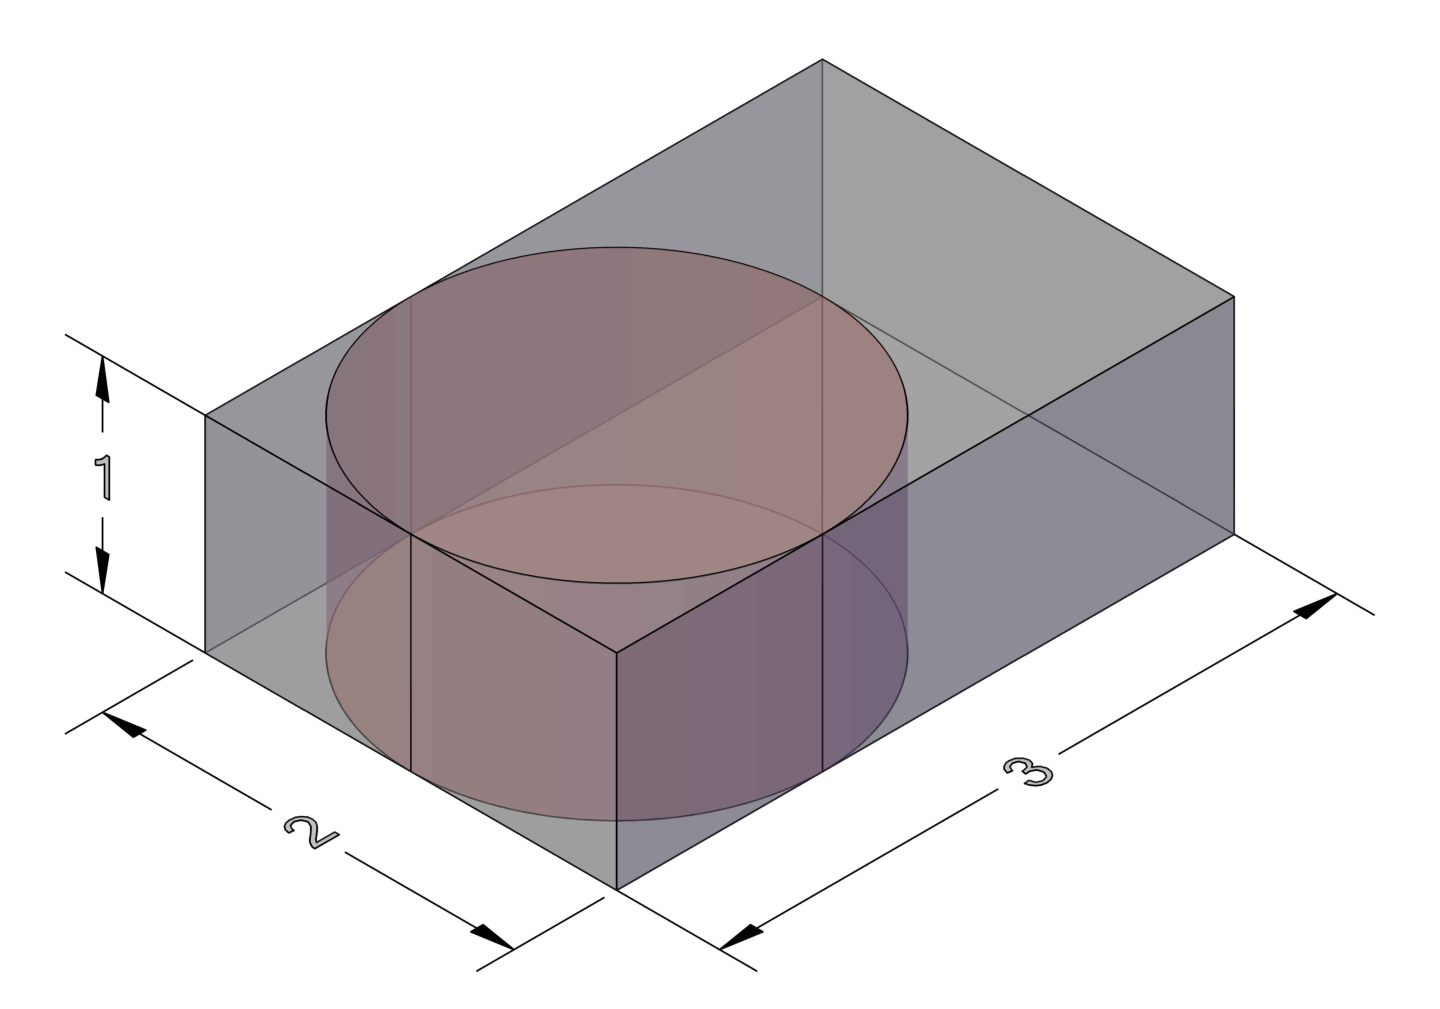
\includegraphics[width=0.30\linewidth]{img/xyInductorCropped.pdf}
    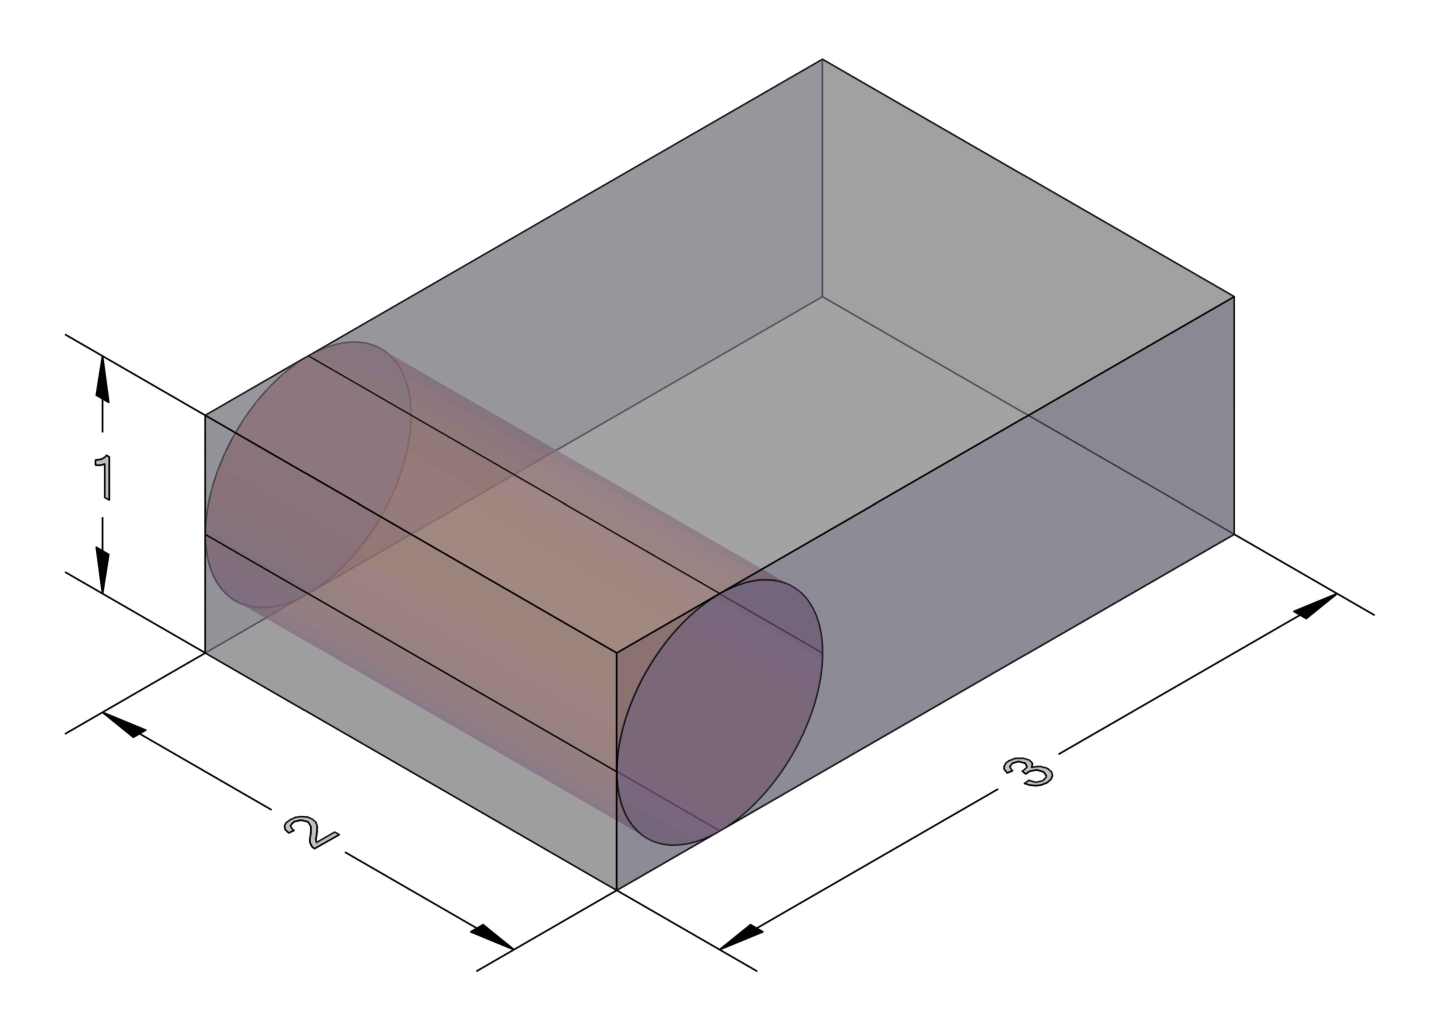
\includegraphics[width=0.30\linewidth]{img/xzInductorCropped.pdf}
    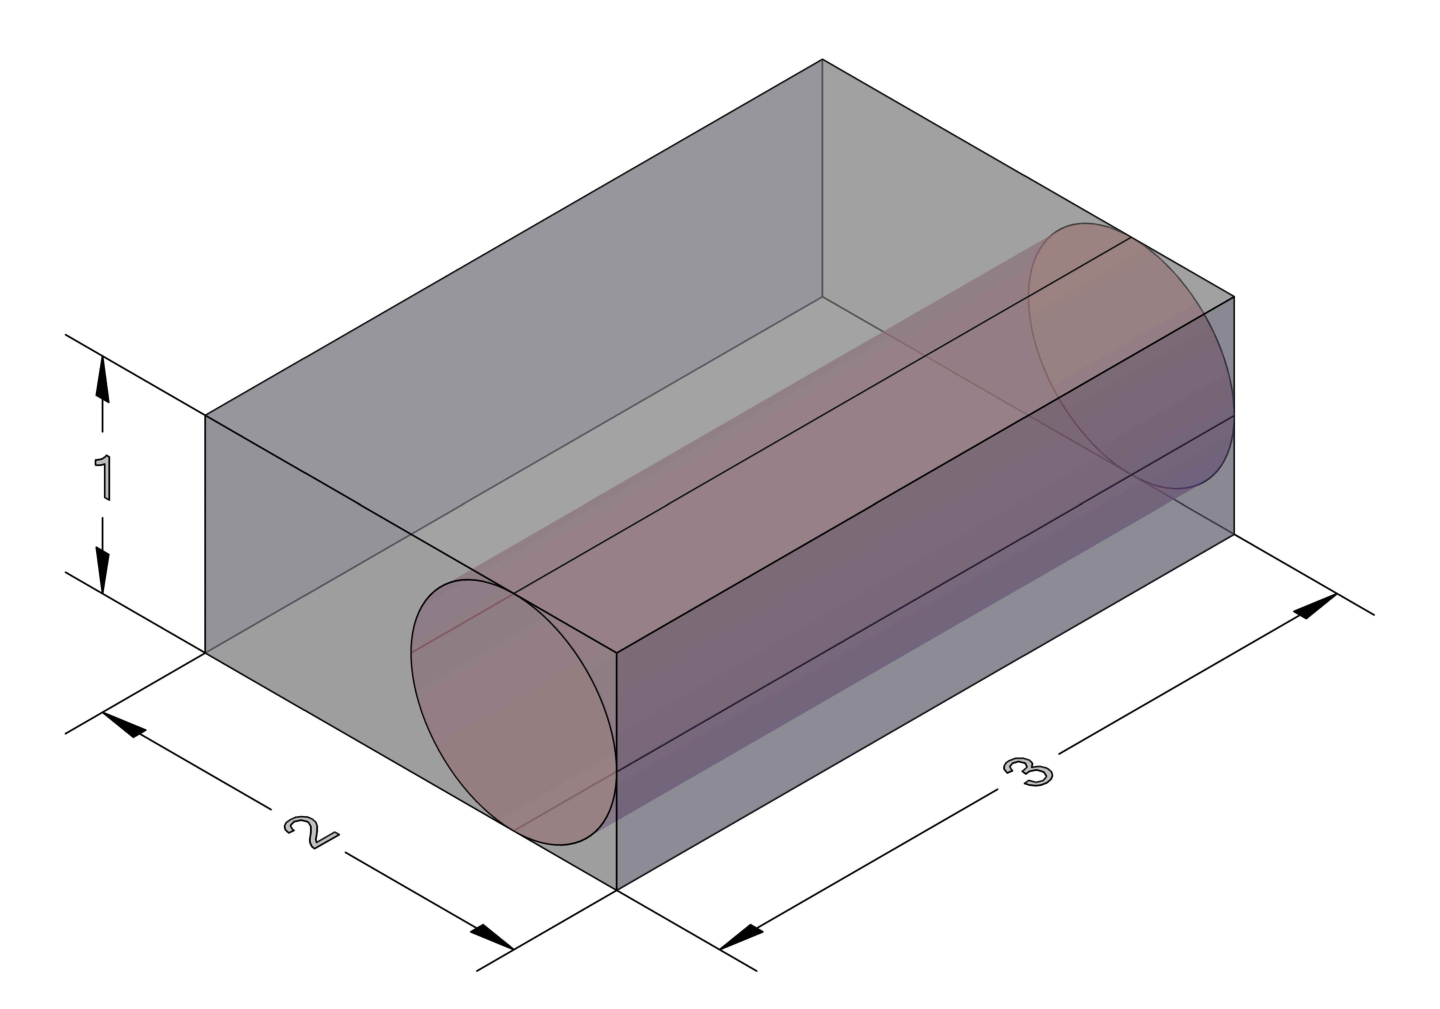
\includegraphics[width=0.30\linewidth]{img/yzInductorCropped.pdf}
    \caption{Inductor Orientation Visualization}Possible orientations of air-core, solenoid-style inductors in a constrained space
    \label{fig:PossibleOrientations}
\end{figure}

\clearpage
%%%%%%%%%%%%%%%%%%%%%%%%%%%%%%
%%%	WITH BIBTEX
%%%%%%%%%%%%%%%%%%%%%%%%%%%%%%
\section*{REFERENCES}

%Add table of contents marker for References
\addcontentsline{toc}{section}{References}

%Add bibliography
\bibliography{bib/mybib} %Replace "bib/mybib" with your directory/bibliography

%Bibliography style
\bibliographystyle{abbrv}

\clearpage
\section*{ABSTRACT}
\addcontentsline{toc}{section}{Abstract}
\centerline{\bf TRADING UTILIZATION FOR CIRCUITRY}
\vspace{-0.4cm}
\centerline{\bf HARDWARE-SOFTWARE CO-DESIGN FOR REAL-TIME}
\vspace{-0.4cm}
\centerline{\bf SOFTWARE-BASED SHORT-CIRCUIT PROTECTION}

{\setlength\baselineskip{0.3in}
\begin{center}
by\\
\medskip
{\bf AARON WILLCOCK}\\
\medskip
{\bf May 2019}\\
\end{center}
\Vspc
\begin{tabular}{ll}
	{\bf Advisor:} & Dr. Nathan Fisher \\
	{\bf Major:} & Computer Science \\
	{\bf Degree:} & Master of Science
\end{tabular}
}

\bigskip \bigskip

Short-circuit faults are a potential source of damage to circuitry in DC-powered systems. Industrial applications including power converters, inverters, and insulated-gate bipolar transistors (IGBTs) often rely on fault protection systems in the form of dedicated circuitry to prevent damage. To increase flexibility in short-circuit protection and decrease dedicated circuitry, a software-based approach is presented. This implementation requires minimal circuitry and allows for trade-off between board space and processor utilization. The design relies on a single inductor and microprocessor running a real-time task for identifying current and monitoring circuitry for faults. Experiments demonstrate detection of both hard-switching faults (HSF) and fault under load (FUL) shorts. The depicted relationship between processor utilization and board space consumed by the circuitry is confirmed through experimentation and allows optimization of board space with respect to utilization and vice versa. As a result, the proposed software-based protection is implementable with the addition of a single component and protects against damage from both HSF and FUL shorts.

\clearpage
\section*{AUTOBIOGRAPHICAL STATEMENT}
\addcontentsline{toc}{section}{Autobiographical Statement}
I am a Ph.D. student in Wayne State University's Department of Computer Science with a focus in real-time systems and a minor in Mechanical Engineering. I help advance real-time, safety-critical systems through research; provide education in computer science ethics through university teaching; and facilitate robotics education through volunteering at local high schools and robotics competitions.

\end{document}

